%%%%%%%%%%%%%%%%%%%%%%%%%%%%%%%%%%%%%%%%%%%%%%%%%%%%%%%%%%%%%%%%%%%%%%%%%%%%%%%
% Copyright (C) 2016  Dale V. Patterson (wraith.wireless@yandex.com)
%
%This program is free software: you can redistribute it and/or modify it under
%the terms of the GNU General Public License as published by the Free Software
%Foundation, either version 3 of the License, or (at your option) any later
%version.
%
%Redistribution and use in source and binary forms, with or without modifications,
%are permitted provided that the following conditions are met:
% o Redistributions of source code must retain the above copyright notice, this
%   list of conditions and the following disclaimer.
% o Redistributions in binary form must reproduce the above copyright notice,
%   this list of conditions and the following disclaimer in the documentation
%   and/or other materials provided with the distribution.
% o Neither the name of the orginal author Dale V. Patterson nor the names of any
%   contributors may be used to endorse or promote products derived from this
%   software without specific prior written permission.
%
% __name__ = 'User Guide'
%__license__ = 'GPLv3'
%__version__ = '0.0.4'
%__date__ = 'June 2016'
%__author__ = 'Dale Patterson'
%__maintainer__ = 'Dale Patterson'
%__email__ = 'wraith.wireless@yandex.com'
%__status__ = 'Production'
%%%%%%%%%%%%%%%%%%%%%%%%%%%%%%%%%%%%%%%%%%%%%%%%%%%%%%%%%%%%%%%%%%%%%%%%%%%%%%%

\documentclass[11pt]{article}
\usepackage[utf8]{inputenc}
\setlength{\parindent}{0pt}
\usepackage{graphicx}
\usepackage{listings}
\usepackage{caption}
\usepackage{geometry}
\usepackage{color}
\usepackage{graphicx}
\usepackage[titletoc,toc,title]{appendix}
\usepackage[T1]{fontenc}
 
\definecolor{codegreen}{rgb}{0,0.6,0}
\definecolor{codegray}{rgb}{0.5,0.5,0.5}
\definecolor{codepurple}{rgb}{0.58,0,0.82}
\definecolor{backcolour}{rgb}{0.95,0.95,0.92}

\geometry{left=1.0in,right=1.0in,top=1.0in,bottom=1.0in }

\lstset{
  frame=top,
  frame=bottom,
  basicstyle=\small\normalfont\ ,
  stepnumber=1,
  numbersep=10pt,
  tabsize=2,              
  extendedchars=true,                     
  breaklines=true,
  captionpos=b,
  mathescape=true,
  showspaces=false,           
  showtabs=false,             
  xleftmargin=17pt,
  framexleftmargin=17pt,
  framexrightmargin=17pt,
  framexbottommargin=5pt,
  framextopmargin=5pt,
  showstringspaces=false,
  backgroundcolor=\color{backcolour},   
    commentstyle=\color{codegreen},
    keywordstyle=\color{magenta},
    numberstyle=\tiny\color{codegray},
    stringstyle=\color{codepurple},
    basicstyle=\footnotesize
}

\title{
\includegraphics[scale=1]{logo}\\ PyRIC v0.1.4: User Manual}
\author{Dale V. Patterson\\ wraith.wireless@yandex.com}

\begin{document}
\maketitle
\tableofcontents

\section{About PyRIC}\label{sec:About}
PyRIC (is a Linux only) library providing wireless developers and pentesters the
ability to identify, enumerate and manipulate their system's wireless cards
programmatically in Python. Pentesting applications and scripts written in Python
have increased dramatically in recent years. However, these tools still rely on
Linux command lines tools to setup and prepare and restore the system for use.
Until now. Why use subprocess.Popen, regular expressions and str.find to interact
with your wireless cards? PyRIC is:
\begin{enumerate}
\item \textbf{Pythonic}: No ctypes, SWIG etc. PyRIC redefines C header files as 
Python and uses sockets to communicate with kernel.
\item \textbf{Self-sufficient}: No third-party files used, PyRIC is completely self-
contained
\item \textbf{Fast}: (relatively speaking) PyRIC is faster than using iw through 
subprocess.Popen
\item \textbf{Parseless}: Get the output you without parsing output from iw. Never 
worry about iw updates and rewriting your parsers.
\item \textbf{Easy}: If you can use iw, you can use PyRIC
\end{enumerate}

At it's heart, PyRIC is a Python port of (a subset of) iw and by extension, a
Python port of Netlink w.r.t nl80211 functionality. The original goal of PyRIC
was to provide a simple interface to the underlying nl80211 kernel support,
handling the complex operations of Netlink seamlessy while maintaining a minimum
of "code walking" to understand, modify and extend. But, why stop there? Since
it's initial inception, PyRIC has grown to include ioctl support to replicate
features of ifconfig such as getting or setting the mac address and has recently
implemented rkill support to soft block or unblock wireless cards.\\

While users can utilize libnl.py to communicate directly with the kernel, the
true utility of PyRIC is pyw.py. Like iw, pyw provides an interface/buffer 
between the caller and the kernel, handling all message construction, parsing 
and transfer transparently and without requiring any Netlink knowledge or 
experience. \\

PyRIC does more though: it implements rfkill, allowing users to list, block and 
unblock devices and implements a subset of ifconfig providing users the ability 
to turn cards on/off and set mac and ip addresses. \\

At this time, PyRIC (through pyw, rfkill and device) can:
\begin{itemize}
\item enumerate interfaces and wireless interfaces,
\item get/set regulatory domain,
\item get/set hw address,
\item get/set ip4, netmask and broadcast address
\item identify a radio's chipset and driver,
\item turn device on/off,
\item get supported standards,
\item get supported commands,
\item get supported modes,
\item get dev/phy info on device,
\item get/set mode,
\item add/delete interfaces, and
\item block/unblock devices through rfkill.
\end{itemize}
And, through libnl.py users can extend the above functionality by creating 
additional commands.\\

\subsection{Background}
PyRIC arose out of a need in Wraith (https://github.com/wraith-wireless/wraith)
for Python nl80211/netlink and ioctl functionality. Originally, Wraith used
ifconfig, iwconfig and iw via subprocess.Popen and parsed the output. There
are obvious shortfalls with this method, especially in terms of iw that is
actively changing (revisions break the parser) and I started looking for an
open source alternative. There are several open source projects out there
such as pyroute, pymnl (and the python files included in the libnl source) but
they generally have either not been maintained recently or come with warnings.
I desired a simple interface to the underlying nl80211 kernel support that
handles the complex operations of netlink seamlessy while maintaining a minimum
of "code walking" to understand, modify and extend. I decided to write my own
because I do not need complete netlink functionality, only that provided by
generic netlink and within the nl80221 family. Additionally, for Wraith, I do
not need a full blown port of iw et. al. functionality to Python but only
require the ability to turn a wireless nic on/off, get/set the hwaddr, get/set
the channel, determine some properties of the card and add/delete interfaces.

So, why did I do this and why is it done "this" way? When I first started to
explore the idea of moving away from iw output parsing, I looked at the source
for iw, and existing Python ports. Just to figure out how to get the family id
for nl80211 required reading through five different source files with no
comments. To that extent, I have attempted to keep subclassing to a minimum,
the total number of classes to a minimum, combine files where possible and where
it makes since and keep the number of files required to be open simultaneously
in order to understand the methodology and follow the program to a minimum. One
can understand the PyRIC program flow with only two files open at any time namely,
pyw and libnl. In fact, only an understanding of pyw is required to add additional
commands although an understanding of libnl.py is helpful especially, if for
example, the code is to be extended to handle multicast or callbacks.

\subsection{Naming Conventions}
The terms interface, device and radio are all used interchangeably throughout to 
refer to a network interface controller (NIC). The following terms will always
have one meaning:
\begin{itemize}
\item \textbf{dev} - the device name i.e. wlan0 or eth0 of a NIC, 
\item \textbf{phy} - the physical index of a NIC i.e. the 0 in phy0,
\item \textbf{ifindex} - the interface index of a NIC,
\item \textbf{card} or \textbf{Card} - a NIC abstraction, an object used in pyw 
functions see the following section for a description. 
\end{itemize}

\subsection{Cards}
A Card is merely a wrapper around a tuple t = (phy index,device name,ifindex). 
Since the underlying Netlink calls sometimes require the physical index, sometimes 
the device name, and sometimes the ifindex, pyw functions\footnote{Not all functions 
accept a Card, devinfo() will accept either a Card or a dev and devadd will accept
either a Card or a physical index} take a Card object which doesn't require callers
to know which identifier to use for each function. There are four primary methods 
to creating a Card: 
\begin{enumerate}
\item \textbf{pyw.getcard} returns a Card object from a given dev,
\item \textbf{pyw.devinfo} returns the dict info where info['card'] is the Card 
object. This function will take either a card or a dev
\item \textbf{pyw.devadd} returns a new Card object, 
\item \textbf{pyw.ifaces} returns a list of tuples t = (Card,mode) sharing the 
same phy as a given dev.
\end{enumerate}

A side affect of using Cards is that many of the netlink calls require the ifindex.
The ifindex is found through the use of ioctl, meaning two sockets have to be 
created and two messages have to be sent, received and parsed in order to execute
the command. With Cards, the ifindex is requested for only once. \\

Keep in mind that any identifier (phy, dev, ifindex) can be invalidated outside 
of your control. Another program can rename your interface, that is change the 
dev without your knowledge. Depending on what functions are being used this may 
not be noticed right away as the phy will remain the same. Also for usb devices, 
(if the usb is disconnected and reconnected) will have the same dev but the phy 
and ifindex will be different.

\subsection{Benchmarks}
PyRIC makes use of several "extensions" to speed up pyw functions:
\begin{enumerate}
\item \textbf{Persistent sockets}: pyw provides the caller with functions and 
the ability to pass their own netlink (or ioctl socket) to pyw functions
\item \textbf{One-time request for the nl80211 family id}: pyw stores the family
id in a global variable
\item \textbf{Consolidation} different "reference" values are consolidated in one
class (see the previous section)
\end{enumerate}

\begin{table}
\begin{center}
\begin{tabular}{| l | r | r | r | r|}
\hline
chset & Total & Avg & Longest & Shortest \\
\hline
Popen(iw) & 588.3059 & 0.0588 & 0.0682 & 0.0021 \\
\hline
one-time & 560.3559 & 0.0560 & 0.0645 & 0.0003 \\
\hline
persistent & 257.8293 & 0.0257 & 0.0354 & 0.0004 \\
\hline
\end{tabular}
\caption{Benchmark: Popen(iw) vs pyw} 
\end{center}
\label{tab:benchmark}
\end{table}

While small, these changes can improve the performance of any programs using pyw. 
Table 1 shows benchmarks for hop time on an Alfa AWUS036NH conducted 10000 times. 
Note that we are not implying that PyRIC is faster than iw. Rather, the table 
shows that PyRIC is faster than using Popen to execute iw. Using one-time sockets,
there is a difference of 28 seconds over Popen and iw with a small decrease in 
the average hoptime. Not a big difference. However, the performance increased
dramatically when persistent netlink sockets are used with the total time and 
average hop time nearly halved.

\section{Installing PyRIC}\label{sec:installing}
The easiest way to install PyRIC is through PyPI:\\

    \texttt{sudo pip install PyRIC}\\

You can also install PyRIC from source. The tarball can be downloaded from:

\begin{itemize}
\item PyPi: https://pypi.python.org/pypi/PyRIC,
\item PyRIC Web: http://wraith-wireless.github.io/PyRIC, or
\item Github: https://github.com/wraith-wireless/PyRIC.
\end{itemize}

After downloading, extract and run:\\

	\texttt{sudo python setup.py install}\\

If you just want to test PyRIC out, download your choice from above. After 
extraction, move the pyric folder (the package directory) to your location of 
choice and from there start Python and import pyw. It is very important that you
do not try and run it from PyRIC which is the distribution directory. This will 
break the imports pyw.py uses. \\

You will only be able to test PyRIC from the pyric directory but, if you want to,
you can add it to your Python path and run it from any program or any location.
To do so, assume you untared PyRIC to /home/bob/PyRIC. Create a text file named
pyric.pth with one line \\

    /home/bob/PyRIC \\

and save this file to /usr/lib/python2.7/dist-packages (or 
/usr/lib/python3/dist-packages if you want to try it in Python 3).

\begin{table}
\begin{center}
\begin{tabular}{| l | r | r | r |}
\hline
Source & Stability & Recency & Installation \\
\hline
pip & 5 & 3 & 5\\
\hline
PyPI & 5 & 3 & 4\\
\hline
PyRIC Web & 4 & 4 & 4\\
\hline
Github & 3 & 5 & 3\\
\hline
\end{tabular}
\caption{Stability vs Recency vs Installation}
\end{center}
\label{tab:install}
\end{table}

\section{Using PyRIC}\label{sec:using}
As stated previously, PyRIC provides a set of functions to interact with your 
system's radio(s) and the ability to interact directly with the kernel through
netlink and ioctl sockets.

\subsection{Interacting with the Wireless Core and Wireless NICs: pyw.py}
If you can use iw, you can use pyw. The easist way to explain how to use pyw is 
with an example. Imagine your wireless network, on ch 6, has been experiencing 
difficulties lately and you want to capture some traffic to analyse it. Listing 
\ref{lst:pentest} shows how to set up a wireless pentest environment. \\

\begin{lstlisting}[caption={Setting up a Wireless Pentest Environment},
                   label={lst:pentest},
                   language=Python]
 1: import pyric                            # pyric error (and ecode EUNDEF)
 2: from pyric import pyw                   # for iw functionality
 3: import pyric.utils.hardware as hw       # for chipset/driver
 4: from pyric.utils.channels import rf2ch  # rf to channel conversion
 5:
 6: dev = 'wlan0'
 7: ifaces = pyw.interfaces()
 8: wifaces = pyw.winterfaces()
 9: if dev not in ifaces:
10:     print "Device {0} is not valid, use one of {1}".format(dev,ifaces)
11:     return
12: elif dev not in wifaces:
13:     print "Device {0} is not wireless, use one of {1}".format(dev,wifaces)
14:
15: print "Regulatory Domain currently: ", pyw.regget()
16: dinfo = pyw.devinfo(dev)
17: card = dinfo['card']
18: pinfo = pyw.phyinfo(card)
19: driver = hw.ifdriver(card.dev)
20: chipset = hw.ifchipset(driver)
21:
22: pyw.down(card)
23: pyw.macset(card,'00:03:93:57:54:46')
24:
25: msg = "Using {0} currently in mode: {1}\n".format(card,dinfo['mode'])
26: msg += "\tDriver: {0} Chipset: {1}\n".format(driver,chipset)
27: if dinfo['mode'] == 'managed':
28:     msg += "\ton channel {0} width {1}\n".format(rf2ch(dinfo['RF']),
29:                                                  dinfo['CHW'])
30: msg += "\tSupports modes {0}\n".format(pinfo['modes'])
31: msg += "\tSupports commands {0}".format(pinfo['commands'])
32: msg += "\thw addr {0}".format(pyw.macget(card))
33: print msg
34:
35: pdev = 'pent0'
36: for iface in pyw.ifaces(card):
37:     pyw.devdel(iface[0])
38: pcard = pyw.devadd(card, pdev, 'monitor')
39: pyw.up(pcard)
40: pyw.chset(pcard,6,None)
41: 
42: # DO STUFF HERE 
43:
44: pyw.devdel(pcard)
45:
46: card = pyw.devadd(card,card.dev,dinfo['mode'])
47: pyw.macset(card,dinfo['mac'])
48: pyw.up(card)
\end{lstlisting}

Listing \ref{lst:pentest} attempts to show most of the available pyw functions 
in use and is the basic shell used in another project, Wraith\cite{wraith}, to 
instantiate a wireless (802.11) sensor - (for a full listing of all pyw functions
see Appendix \ref{sec:pywapi}) - with scanning capabilities. Lines 1 and 2 should 
always be included as they import the pyric error and pyw functions. Line 3 
imports hardware which provides the ifchipset and ifdriver functions and Line 4 
imports the rf2ch conversion function. \\

In lines 6 through 13, the device wlan0 is confirmed wireless and lines 16 through
20 a Card object for 'wlan0' is created and details about the interface are printed. 
Next, the mac address of wlan0 is changed on lines 23. Note, the device is brought
down first. \\

More information on the device is printed in lines 25 through 33. Starting on
line 35, a device named 'pent0' is created in monitor mode. First in lines 36 
and 37, all interfaces on the same phy are deleted \footnote{we have found that
it is better to delete all interfaces on the same phy ensuring that external 
processes don't interfere with the new device} before creating the new device, 
bringing the card up and setting it to channel 6 NOHT.\\ 

Restoring the device starts on line 45, where the virtual interface is deleted,
the previous interface is restored and the mac address is reset.

\subsubsection{One-time vs Persistent Sockets}
The example in Listing \ref{lst:pentest} uses one-time sockets (netlink and 
ioctl). When using iw, there are several things that occur prior to the actual 
command or request being submitted. First, iw creates a netlink socket. Then, 
iw will request the family id for nl80211. The relative time spent doing this 
is neglible but, it is redundant and it may become noticeable in programs that
repeatedly use the Netlink service. Once comlete, iw closes the socket. In some
cases, the ifindex of the device is needed and iw will also initiate an ioctl 
call to retrieve it. PyRIC eliminates these redundancies by using a global 
variable in pyw that stores the family id after the first time it is requested 
and by providing callers the option to use persistent sockets. 
\begin{itemize}
\item \textbf{One-time Sockets} Similar to iw. The command, creates the netlink 
socket (or ioctl socket), composes the message, sends the message and receives 
the response, parses the results, closes the socket and returns the results to 
the caller. At no time does the caller need to be aware of any underlying Netlink 
processes or structures.
\item \textbf{Persistent Sockets} Communication and parsing only. The onus of 
socket creation and deletion is on the caller which allows them to create one 
(or more) socket(s). The pyw functions will only handle message construction, 
message sending and receiving and message parsing.
\end{itemize}
The caller needs to be cognizant of whether the function requires a netlink or
ioctl socket. Passing the wrong type will result in an error. \\

NOTE: One must remember that there is an upper limit to the number of open netlink
sockets. It is advised to use one-time functions as much as possible and save the
use of persistent sockets for use in code that repeatedly makes use of netlink. \\

The latest version of pyw.py (v 0.1.*) implements this functionality through the 
use of what I call templates\footnote{I use templates and stubs for the lack
of any better naming convention}, Listing \ref{lst:template} and stubs Listing 
\ref{lst:stub}.

\begin{lstlisting}[caption={A Basic Netlink Function Template},
                   label={lst:template},
                   language=Python]
def fcttemplate(arg0,arg1,..,argn,*argv):
    # put parameter validation (if any) here
    try:
        nlsock = argv[0]
    except IndexError:
        return _nlstub_(fcttemplate,arg0,arg1,...,argn)
        
    # command execution
    ...
    return results
\end{lstlisting}

The template function in Listing \ref{lst:template} checks if argv has a netlink
socket\footnote{ioctl calls operate in the same manner} at index 0. If so, it
proceeds to execution. If there is no socket, the stub is executed which creates 
one. If something other than a netlink socket is at argv[0], an error will be 
raised during execution. \\

\begin{lstlisting}[caption={Function \_nlstub\_},
                   label={lst:stub},
                   language=Python]
def _nlstub_(fct,*argv):
    nlsock = None
    try:
        nlsock = nlsock = nl.nl_socket_alloc()
        argv = list(argv) + [nlsock]
        return fct(*argv)
    except pyric.error: 
        raise # catch & release
    finally:
        if nlsock: nl.nl_socket_free(nlsock)
\end{lstlisting}

The stub function, Listing \ref{lst:stub} allocates a netlink socket, executes
the original (now with a netlink socket) and then destroys the netlink socket.\\

\begin{lstlisting}[caption={Using Persistent Sockets},
                   label={lst:persistent},
                   language=Python]
 1: import pyric                      # pyric error (and ecode EUNDEF)
 2: from pyric import pyw             # for iw functionality
 3: from pyric.lib import libnl as nl # for netlink sockets
 4:
 5: nlsock = nl.nl_socket_alloc(timeout=1)
 6: card = pyw.getcard('wlan0',nlsock)
 7: print pyw.devmodes(card,nlsock)
 8: nl.nl_socket_free(nlsock)
\end{lstlisting}

Listing \ref{lst:persistent}, shows the creation of a persistent netlink socket 
that is used in the creation of a card and in retrieved the card's supported
modes. \\

Use Python's built in help features on pyw functions or see Appendex \ref{sec:pywapi} 
to determine what type of socket is needed.

\subsection{Additional Tools}
In the utils directory, PyRIC includes channels.py, hardware.py, rfkill.py and
ouifetch.py. These provide a port of rfkill, channel/frequency enumeration and 
device chipset, driver retrieval as well as some mac address functions. More 
information can be found in the Appendices and in README.md. 

\subsection{Interacting with the Kernel: libnl.py and libio.py}
The kernel interfaces, libnl.py and libio.py are located in the lib directory.
They handle socket creation/deletion, message creation/parsing and kernel 
communication. Aside from creating and deleting persistent sockets, there is 
little need to access their functions unless you plan on extending pyw 
functionality. As such, a further discussion of libnl.py and libio.py can be 
found in the next section.   

\section{Extending PyRIC}\label{sec:extending}
You may find that pyw does not offer some of the functionality you need. Using
libnl.py and/or libnl.io, additional functionality can be added to your program.\\ 

It is helpful if the reader has a basic knowledge of netlinks. For a review, see 
"Communicating between the kernel and user-space in Linux using Netlink Sockets"
\cite{spae}. 

\subsection{Porting C}
All Python ports of C header files can be found in the net directory. C Enums 
and \#defines are ported using constants. C structs are ported using three 
Python structures and the Python struct package:
\begin{enumerate}
\item a format string for packing and unpacking the struct
\item a constant specifying the size of the struct in bytes
\item a function taking the attributes of the struct as arguments and returning
a packed string
\end{enumerate}
Listing \ref{lst:cstruct} shows the C definition of the nlmsghdr found in netlink.h.

\begin{lstlisting}[caption={C Struct nlmsghdr},
                   label={lst:cstruct},
                   language=C]
struct nlmsghdr {
    __u32 nlmsg_len;
    __u16 nlmsg_type;
    __u16 nlmsg_flags;
    __u32 nlmsg_seq;
    __u32 nlmsg_pid;
};
\end{lstlisting}

And Listing \ref{lst:pstruct} shows the ported version in Python.

\begin{lstlisting}[caption={Corresponding Python Definition},
                   label={lst:pstruct},
                   language=Python]
nl_nlmsghdr = "IHHII"
NLMSGHDRLEN = struct.calcsize(nl_nlmsghdr)
def nlmsghdr(mlen,nltype,flags,seq,pid):
    return struct.pack(nl_nlmsghdr,NLMSGHDRLEN+mlen,nltype,flags,seq,pid)
\end{lstlisting}

When using pyw, dealing with these structures is handled transparently by libnl.py 
and libio.py. When extending or customizing pyw, a basic understanding of the 
definitions in netlink\_h.py, genetlink\_h.py and if\_h.py.

\subsection{Input/Output Control (ioctl)}
PyRIC provides more than just iw-related functions, it also implements functions
from ifconfig and iwconfig. These command line tools still use ioctl (or the proc
directory). For example, interfaces() reads from '/proc/net/dev' to retrieve all
system interfaces and winterfaces() use ioctl to check if a device is wireless.
Input/Output control calls have only been used when there was no viable alternative 
and, it should not be necessary to have to add any further ioctl commands. If you
find that you need an ioctl related command, search through if\_h.py for the 
appropriate structure and add it's definitions to ifreq. 

\subsection{Netlink and nl80211}
Documentation on Netlink, and nl80211 in particular, is so minimal as to be 
neglible. The clusterfuck of code and lack of comments in the iw source tree 
make it impossible to use as any sort of roadmap. Fortunately Thomas Graf's 
site\cite{libnl} has excellent coverage of libnl, the Netlink library. Using 
this as a reference, a simple Netlink parser was put together which later became
libnl.py. Using the command line tool strace and libnl.py, Netlink messages could
be dissected and analyzed.\\

Let us consider adding a virtual interface with the command:\\

    \texttt{sudo iw phy0 interface add test0 type monitor}\\
    
First, we need to see what is going on under the covers. Using strace:\\

    \texttt{strace -f -x -s 4096 iw phy0 interface add test0 type monitor}\\  

from a terminal will give a you a lot of output, most irrelevant (to us). Scroll
through this until the netlink socket creation as highlighted in Figure
\ref{fig:nlsock}. You can see that a socket of type PF\_NETLINK is created and
the send/receive buffers are set to 32768.
\begin{center}
\begin{figure}[h]
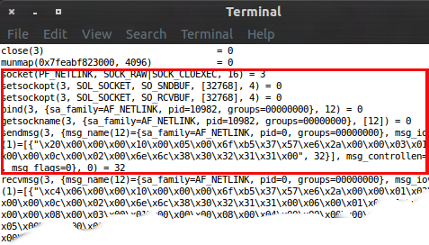
\includegraphics{nlsock}
\caption{Netlink socket creation}
\label{fig:nlsock}
\end{figure}
\end{center} 
What we want to analyze are the messages sent and received over the netlink 
socket. In Figure \ref{fig:nlsock}, iw is requesting the family id for nl80211. 
This id will be used in subsequent requests related to nl80211 as we will see 
shortly. The return message gives the nl80211 family id as 26 and returns other
nl80211 attributes. This is handled by the private function \_familyid\_ in 
pyw.py.

Figure \ref{fig:nlsend} shows the add interface message being sent to the kernel.
\begin{center}
\begin{figure}[h]
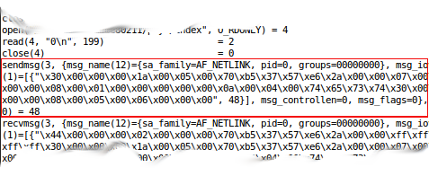
\includegraphics{nlsend}
\caption{Netlink sendmsg}
\label{fig:nlsend}
\end{figure}
\end{center} 
We are interested in the byte sequence following msg\_iov(1). Copy this and paste
into in a python variable as in Listing \ref{lst:nlparse} and pass it to the
function nlmsg\_fromstream which parses the byte stream and returns the GENLMsg.\\

\begin{lstlisting}[caption={Parsing netlink messages},
                   label={lst:nlparse},
                   language=Python]
>>> from pyric.lib import libnl as nl
>>> sent = "\x30\x00\x00\x00\x1a...\x00\x00"
>>> msg = nl.nlmsg_fromstream(sent)
>>> msg
nlmsghdr(len=48,type=26,flags=5,seq=1463268720,pid=10982)
genlmsghdr(cmd=7)
attributes:
	0: type=1,datatype=3
	value=0
	1: type=4,datatype=5
	value=test0
	2: type=5,datatype=3
	value=6
\end{lstlisting}

The first thing to notice is nlmsghdr type = 26, which of course is nl80211 family
id. The rest of the nlmsghdr components len, flags, seq, and pid are handled by
libnl.py although you can supply your own flags if desired. At this time, you can
manually look up what values the cmd, type and datatype correspond to in 
nl80211\_h.py and netlink\_h.py or you can use the tools provided in nlhelp.py.\\

\begin{lstlisting}[caption={Parsing netlink messages continued},
                   label={lst:nlparse2},
                   language=Python]
>>> from pyric.net.netlink_h import NLA_DATATYPES
>>> from pyric.docs import nlhelp
>>> nlhelp.cmdbynum(7)
u'@NL80211_CMD_NEW_INTERFACE'
>>>
>>> for attr in msg.attrs:
...     print nlhelp.attrbynum(attr[0]), NLA_DATATYPES[attr[2]], attr[1]
... 
@NL80211_ATTR_WIPHY u32 0
@NL80211_ATTR_IFNAME string test0
@NL80211_ATTR_IFTYPE u32 6
>>>
>>> from pyric.net.wireless.nl80211_h import NL80211_IFTYPES
>>> NL80211_IFTYPES[6]
'monitor'
\end{lstlisting}

In Listing \ref{lst:nlparse2} command number 7 corresponds to 
NL80211\_CMD\_NEW\_INTERFACE and the attributes that need to be passed to the
kernel are NL80211\_ATTR\_WIPHY, NL80211\_ATTR\_IFNAME and NL80211\_ATTR\_IFTYPE.
The IFTYPE is also known as the mode i.e. 'monitor' which can be found in
nl80211\_h.py NL80211\_IFTYPES. We don't parse the return message from the kernel
but, it follows the same SOP. In this case, it returns the attributes of the new
virtual interface. \\

With this information, we can now code our function. Recall the fcttemplate as
defined in Listing \ref{lst:template} and fill in the command execution as shown 
in Listing \ref{lst:coding}. \\

\begin{lstlisting}[caption={Coding the function},
                   label={lst:coding},
                   language=Python]
# construct the message
msg = nl.nlmsg_new(nltype=_familyid_(nlsock),
                   cmd=nl80211h.NL80211_CMD_NEW_INTERFACE,
                   flags=nlh.NLM_F_REQUEST | nlh.NLM_F_ACK)
nl.nla_put_u32(msg,card.phy,nl80211h.NL80211_ATTR_WIPHY)
nl.nla_put_string(msg,vdev,nl80211h.NL80211_ATTR_IFNAME)
nl.nla_put_u32(msg,IFTYPES.index(mode),nl80211h.NL80211_ATTR_IFTYPE)

# send, receive and parse return results, returning the new Card
nl.nl_sendmsg(nlsock,msg)
rmsg = nl.nl_recvmsg(nlsock) # success returns new device attributes
return Card(card.phy,vdev,nl.nla_find(rmsg,nl80211h.NL80211_ATTR_IFINDEX))
\end{lstlisting}

We construct a new GENLMsg passing the nl80211 family id, the command we got
earlier and flags specifying that this is a request and we want to get an ACK
back\footnote{libnl.py always forces an ACK and handles the underlying process 
of receiving it}. Now, add each attribute to the message. Note the order: value, 
then attribute. With the message constructed, send it to the kernel, get the 
results, parse and return them.\\

Rather simple, in fact the hardest part is figuring out what to send to the kernel.
Everything else is handled behind the scenes by libnl.py.

\begin{appendices}
\section{API: pyw.py}\label{sec:pywapi}

\subsection{Constants}
\begin{itemize}
\item \textbf{\_FAM80211ID\_}: Global netlink family id of nl80211. Do not touch
\item \textbf{IFTYPES}: redefined (from nl80211\_h.py) interface modes
\item \textbf{MNTRFLAGS}: redefined (from nl80211\_h.py) monitor mode flags
\item \textbf{IPADDR}: Regular Expression for ip4 address validation
\item \textbf{MACADDR}: Regular Expression for mac address validation
\end{itemize}

\subsection{Objects/Classes}
\textbf{Card} A wrapper around a tuple 
\texttt{t = (physical index,device name,interface index)}
which exposes the following properties through '.':
\begin{itemize}
\item \textbf{phy}: physical index
\item \textbf{dev}: device name
\item \textbf{idx}: interface index (ifindex)
\end{itemize}
Because the underlying Netlink calls will sometimes require the physical index,
sometimes the device name, and sometimes the ifindex, pyw functions accept a Card,
object. This allows callers to use pyw functions without having to remember which 
identifier the function requires. However, in some cases the function requires 
a dev or accepts both. See the next section on functions.\\

While callers could create their own Cards, it is recommend to use one of the 
following
\begin{itemize}
\item \textbf{pyw.getcard} returns a Card object from a given dev
\item \textbf{pyw.devinfo} returns the dict info where info['card'] is the Card 
object. This function will take either a card or a dev
\item \textbf{pyw.devadd} returns a new Card object
\item \textbf{pyw.ifaces} returns a list of tuples t = (Card,mode) sharing the 
same phy as a given device to do so. It is also recommended to periodically 
validate the Card. On some cheaper usb wireless nics, there are periodic 
disconnects which results in a new phy and ifindex.
\end{itemize}

\subsection{Functions}
\begin{itemize}
\item interfaces(): (ifconfig), type: filesystem, returns list of all network dev
\item isinterface(dev): (ifconfig <dev>) type: filesystem, check dev is an interface
\item winterfaces([iosock]): (iwconfig), type: ioctl, list wireless interfaces
\item iswireless(dev,[iosock]): (iwconfig <dev>), type: ioctl, check dev is a 
wireless interface
\item regget([nlsock]: (iw reg get), type: netlink, get regulatory domain
\item regset(rd,[nlsock]): (iw reg set <rd>), type: netlink, set regulatory domain 
to rd
\item getcard(dev,[nlsock]) (N/A), type: hybrid netlink and ioctl: get a Card 
object for dev
\item validcard(card,[nlsock]): (N/A), type: (hyrbrid netlink and ioctl), verify
card is still valid
\item macget(card,[iosock]): (ifconfig), type: ioctl, determine if card is up
or down
\item macset(card,mac,[iosock]): (ifconfig card.<dev> hw ether <mac>), type: 
ioctl, set card's hw address to mac
\item isup(card,[iosock]): (ifconfig card.<dev>) 
\item up(card,[iosock]) (ifconfig card.<dev> up), type: ioctl, bring card up
\item down(card,[iosock]): (ifconfig card.<dev> down), type: ioctl, bring card 
down
\item isblocked(card): (rfkill list <rfkill\_idx>): type N/A returns tuple 
(Soft Block State, Hard Block State) 
\item block(card): (rfkill block <rfkill\_idx>) type: N/A, soft blocks card
\item unblock(card): (rfkill unblock <rfkill\_idx>) type: N/A, removes the soft 
block on card
\item pwrsaveget(card,[nlsock]) (iw dev card.<dev> get power\_save) type: netlink
get card's power save state True = on, False = off
\item pwrsaveset(card,on,[nlsock]) (iw dev card.<dev> set power\_save <on>) type:
netlink set card's power save state True = on, False = off
\item covclassget(card,[nlsock]) (iw phy card.<phy> get coverage <cc>) type:
netlink get card's coverage class
\item covclassset(card,cc,[nlsock]) (iw phy card.<phy> set coverage <cc>) type:
netlink set card's coverage class
\item retryshortget(card,[nlsock]) (iw phy card.<phy> info | grep 'retry short')
type:netlink get card's retry short limit
\item retryshortset(card,lim,[nlsock]) (iw phy card.<phy> set retry short <lim>)
type:netlink set card's retry short limit
\item retrylongget(card,[nlsock]) (iw phy card.<phy> info | grep 'retry long')
type:netlink get card's retry long limit
\item retrylongset(card,lim,[nlsock]) (iw phy card.<phy> set retry long <lim>)
type:netlink set card's retry long limit
\item rtsthreshget(card,[nlsock]) (iw phy card.<phy> info | grep rts) type: 
netlink set card's RTS threshold
\item rtsthreshset(card,thresh,[nlsock]) (iw phy card.<phy> set rts <thresh>) type: 
netlink set card's RTS threshold
\item fragthreshget(card,[nlsock]) (iw phy card.<phy> info | grep frag) type: 
netlink get card's fragmentation threshold
\item fragthreshset(card,thresh,[nlsock]) (iw phy card.<phy> set frag <thresh>) type: 
netlink set card's fragmentation threshold
\item inetget(card,[iosock]): (ifconfig card.<dev>), type: ioctl, get ip4 address,
netmask and broadcast address of card
\item inetset(card,ipaddr,netmask,broadcast,[iosock]): (ifconfig card/<dev> <ipaddr>
netmask <netmask> broadcast <broadcast>), type: ioctl, set the interface addresses
of the card
\item ip4set(card,ipaddr,[iosock]): (ifconfig card.<dev> <ipaddr>), type: ioctl,
set the card's ip4 address
\item netmaskset(card,netmask,[iosock]): (ifconfig card.<dev> netmask <netmask>), 
type: ioctl, set the card's netmask
\item broadcastset(card,broadcast,[iosock]): (ifconfig card.<dev> broadcast 
<broadcast>), type: ioctl, set the card's broadcast address
\item devfreqs(card,[nlsock]): (iw phy card.phy info), type: netlink, get card's 
supported frequencies
\item devchs(card,[nlsock]): (iw phy card.phy info), type: netlink, get card's 
supported channels
\item devstds(card,[iosock]): (iwconfig card.<dev> | grep IEEE), type: ioctl, get
list of card's 802.11 supported standards
\item devmodes(card,[nlsock]): (iw phy card.phy info | grep interface), type:
netlink, get card's supported modes
\item devcmds(card,[nlsock]): (iw phy card.phy info | grep commands), type:
netlink, get card's supported commands
\item devinfo(card,[nlsock]): (iw dev card.<dev> info), type: netlink, get info 
for dev 
\item phyinfo(card,[nlsock]): (iw phy card.<phy> info), type: netlink, get info
for phy
\item ifaces(card,[nlsock]): (APX iw card.dev | grep phy\#), type: netlink, get all
cards (w/ modes) of interfaces sharing the same phy as card
\item txset(card,pwr,lvl,[nlsock]) (iw phy phy0 set txpower <lvl> <pwr>), type: 
netlink,sets the tx power to pwr (in dBm) with level setting lvl 
\item txget(card,[iosock]): (iwconfig card.<dev> | grep Tx-Power card), type: 
ioctl, get card's transmission power
\item chget(card,[nlsock]): (iw dev <card.dev> info | grep channelS), type: 
netlink, get card's current channel (only works for cards in mode managed)
\item chset(card,ch,chw,[nlsock]): iw phy <card.phy> set channel <ch> <chw>), 
type: netlink, set card's current channel to ch with width chw
\item freqset(card,rf,chw,[nlsock]): iw phy <card.phy> set freq <rf> <chw>), 
type: netlink, set card's current frequency to rf with width chw
\item devmodes(card,[iosock]): (iw phy card.<phy>), type: netlink, get modes 
supported by card
\item modeset(card,mode,[flags],[nlsock]): (iw dev card.<dev> set type <mode> 
[flags]), type: netlink, set card's mode to mode with flags (if mode is monitor)
\item modeget(card[nlsock]): (iw dev card.<dev> info | grep mode), type: netlink,
get card's mode
\item devadd(card,vnic,mode,[flags],[nlsock]): (iw phy card.<phy> interface add
<vnic> type <mode> flags <flags>), type: netlink, creates a new virtual interface
on card's phy with dev vdev, in mode and using flags. Note: flags are only supported
in when creating a monitor mode
\item devdel(card,[nlsock]): (iw card.<dev> del), type: netlink, deletes dev
\begin{itemize}
\item \_hex2mac\_(v): returns a ':' separated mac address from byte stream v
\item \_hex2ip4\_(v): returns a '.' separated ip4 address from byte stream v
\item \_validip4\_(addr): determines if addr is a valid ip4 address
\item \_validmac\_(addr): determines if addr is a valid mac address
\item \_issetf\_(flags,flag): determines if flag is set in flags
\item \_setf\_(flags,flag): set flag in flags to on
\item \_unsetf\_(flags,flag): set flag in flags to off
\item \_familyid\_(nlsock): returns and sets the Netlink family id for nl80211, 
only called once per module import
\item \_ifindex\_(dev,[iosock]): returns dev's ifindex
\item \_flagsget\_(dev,[iosock]): get's the dev's interface flags
\item \_flagsset\_(dev,flags,[iosock]): set's the dev's interface flags
\item \_iftypes\_(i): returns the mode corresponding to i
\item \_frequencies\_(band): returns a list of frequencies from the packed byte 
string band
\item \_commands\_(command): converts the list of numeric commands to a list of
commands as strings 
\item \_ciphers\_(cipher): returns a list of ciphers from the packed byte string
cipher
\item \_iostub\_(fct,*argv): ioctl stub function, calls fct with parameter list argv
and an allocated ioctl socket
\item \_nlstub\_(fct,*argv): netlink stub function, calls fct with parameter list
argv and an allocated netlink socket
\end{itemize}
\end{itemize}

\section{API: channels.py}\label{sec:channels.api}
Channel, Frequency enumeration and conversions can be found in channels.py.

\subsection{Constants}
\begin{enumerate}
\item \textbf{CHTYPES}: imported channel types from nl80211\_h
\item \textbf{CHWIDTHS}: imported channel widths from nl80211\_h
\item \textbf{ISM\_24\_C2F}: Dict containing ISM channel (key) to frequency (value) 
pairs
\item \textbf{ISM\_24\_F2C}: Dict containing ISM frequency (key) to channel (value)
pairs
\item \textbf{UNII\_5\_C2F}: Dict containing UNII 5Ghz channel (key) to frequency 
(value) pairs
\item \textbf{UNII\_5\_F2C}: Dict containing UNII 5Ghz frequency (key) to channel 
(value) pairs
\item \textbf{UNII\_4\_C2F}: Dict containing UNII upper 4Ghz channel (key) to 
frequency (value) pairs
\item \textbf{UNII\_4\_F2C}: Dict containing UNII upper 4Ghz frequency (key) to 
channel (value) pairs
\end{enumerate}

\subsection{Functions}
\begin{enumerate}
\item channels(): returns a list of all channels
\item freqs(): returns a list of all frequencies
\item ch2rf(c): convert channel c to frequency
\item rf2ch(f): convert frequency f to channel
\end{enumerate}

\section{API: hardware.py}\label{sec:hardwareapi}
Hardware related: driver, chipset, manufacturer and mac address utility functions 
can be found in device.py.

\subsection{Constants}
\begin{enumerate}
\item \textbf{dpath}: path to system device details
\item \textbf{drvpath}: path to device drivers 
\end{enumerate}

\subsection{Functions}
\begin{enumerate}
\item oui(mac): returns the oui portion of address <mac>
\item ulm(mac): returns the ulm portion of address <mac>
\item manufacturer(ouis,mac): returns the manufacturer name of <mac> given the
dict of <ouis>
\item randhw([ouis]): returns a random mac address. If the dict ouis is specified 
will select a random oui from the dict otherwise will generate one
\item ifcard(dev): returns the device driver and chipset
\item ifdriver(dev): returns the device driver
\item ifchipset(driver): returns the chipset associated with driver
\end{enumerate}

\section{API: ouifetch.py}
The file ouifetch.py retrieves and saves a tab seperated file of oui to 
manufacturer name for use by hardware.py functions. From a command line, type: \\

\subsection{Constants}
\begin{enumerate}
\item \textbf{OUIURL}: url of IEEE oui file
\item \textbf{OUIPATH}: path to default location PyRIC oui.txt file
\end{enumerate}

\subsection{Functions}
\begin{enumerate}
\item parse([opath]): returns a dict of oui:manufacturer key->value pairs stored
in the text file at opath. If opath is not specified, uses the default
\item fetch([opath]): retrieves oui.txt from the IEEE website, parses the files
and stores the results in a PyRIC friendly format in opath. If opath is not 
specified, uses the default. User must have root permissions in order to write
to default opath 
\end{enumerate}

\section{API: rfkill.py}\label{sec:rfkillapi}
A port of the command line tool rfkill, rfkill.py writes and reads rfkill\_event 
structures to /dev/rfkill using fcntl providing functionality to block and unblock 
devices. 

\subsection{Constants}
\begin{enumerate}
\item \textbf{RFKILL\_STATE}: list of boolean values corresponding to blocked, 
unblocked
\end{enumerate}

\subsection{Functions}
\begin{enumerate}
\item rfkill\_list(): corresponds to rkill list, returns a dict of dicts name -> 
\{idx, type, soft, hard\}. If type is 'wireless', then name will be of the form
phy<n> such that n is the physical index of the wireless card 
\item rfkill\_block(idx): soft blocks the device at rfkill index idx
\item rfkill\_blockby(rtype): soft blocks all devices of type rtype
\item rfkill\_unblock(idx): turns off the soft block at rfkill index idx
\item rfkill\_unblockby(rtype): turns off the soft blocks of all devices of type
rtype
\item soft\_blocked{idx}: determines soft block state of device at rfkill index idx
\item hard\_blocked{idx}: determines hard block state of device at rfkill index idx
\item getidx(phy): returns the rfkill index of the device with physical index phy
\item getname(idx): returns the name of the device at rfkill index idx
\item gettype(idx): returns the type of the device at rfkill index idx
\end{enumerate}

\section{API: libnl.py}\label{sec:libnlapi}
Providing libnl similar functionality, libnl.py provides the interface between
pyw and the underlying nl80211 core. It relates similarily to libnl by providing
functions handling netlink messages and sockets and where possible uses similarly
named functions as those libnl to ease any transitions from C to PyRIC. However,
several liberties have been taken as libnl.py handles only nl80211 generic netlink
messages.

\subsection{Constants}
\begin{itemize}
\item \textbf{BUFSZ} default rx and tx buffer size
\end{itemize}

\subsection{Classes/Objects}
The two classes in libnl.py, NLSocket and GENLMsg, discussed in the following 
sections subclass Python's builtin dict. This has been done IOT to take advantage 
of dict's already existing functions and primarily their mutability and Python's
'pass by name' i.e. modifications in a function will be reflected in the caller.
This makes the classes very similar to the use C pointers to structs in libnl.

\subsubsection{NLSocket}
NLSocket is a wrapper around a netlink socket which exposes the following 
properties through '.':
\begin{itemize}
\item \textbf{sock}: the actual socket
\item \textbf{fd}: the socket's file descriptor (deprecated)
\item \textbf{tx}: size of the send buffer
\item \textbf{rx}: size of the receive buffer
\item \textbf{pid}: port id
\item \textbf{grpm}: group mask 
\item \textbf{seq}: sequence number
\item \textbf{timeout}: socket timeout
\end{itemize}
and has the following methods:
\begin{itemize}
\item incr(): increment sequence number
\item send(pkt): sends pkt returning bytes sent
\item recv(): returns received message (will block unless timeout is set)
\item close(): close the socket
\end{itemize}

NLSockets are created with nl\_socket\_alloc and must be freed with nl\_socket\_free.
See Section \ref{sec:libnlfct}.

\subsubsection{GENLMsg}
GENLMsg is a wrapper around a dict with the following key->value pairs:
\begin{itemize}
\item \textbf{len}: total message length including the header
\item \textbf{nltype}: netlink type
\item \textbf{flags}: message flags
\item \textbf{seq}: seq. \#
\item \textbf{pid}: port id
\item \textbf{cmd}: generic netlink command
\item \textbf{attrs}: list of message attributes. Each attribute is a tuple t =
(attribute,value,datatype) where:
\begin{itemize}
\item \textbf{attribute}: netlink attribute type i.e. CTRL\_ATTR\_FAMILY\_ID
\item \textbf{value}: the unpacked attribute value
\item \textbf{datatype}: datatype of the attribute as defined in nelink\_h i.e.
NLA\_U8
\end{itemize}
\end{itemize}
NOTE: as discussed below, on sending, the seq. \# and port id are overridden with
values of the netlink socket.\\

GENLMsg exposes the following properties:
\begin{itemize}
\item \textbf{len}: length of the message (get only)
\item \textbf{vers}: returns 1 (default version) (get only)
\item \textbf{nltype}: message content i.e. generic or nl80211 (get or set)
\item \textbf{flags}: message flags (get or set)
\item \textbf{seq}: current sequence \# (get or set)
\item \textbf{pid}: port id (get or set)
\item \textbf{cmd}: netlink command (get or set)
\item \textbf{attrs}: attribute list (get only)
\item \textbf{numattrs}: number of attributes (get only)
\end{itemize}

GENLMsg has the following methods:
\begin{itemize}
\item \_\_repr\_\_(): returns a string representation useful for debugging
\item tostream(): returns a packed netlink message

There are two methods of creating a GENLMsg. Create a new message (to send) with 
nlmsg\_new and create a message from a received packet with nlmsg\_fromstream. 
These are discussed below.

\subsection{Functions}\label{sec:libnlfct}
\begin{itemize}
\item \textbf{Netlink Socket Related}
\begin{itemize}
\item nl\_socket\_alloc(pid,grps,seq,rx,tx,timeout): creates a netlink socket 
with port id = pid, group mask = grps, initial seq. \# = seq, send and receive
buffer size = tx and rx respectively and blocking timeout = timeout
\item nl\_socket\_free(sock): closes the socket
\item nl\_socket\_pid(sock): (deprecated for NLSocket.pid) returns the port id
\item nl\_socket\_grpmask(sock): (deprecated for NLSocket.grpmask) returns the 
group mask
\item nl\_sendmsg(sock,msg,override=False): sends the netlink msg over socket. 
NOTE: NLSockets will automatically set the port id and seq. \# regardless of 
their value in the message. If override is True, the message's pid and seq. \# 
will be used instead. 
\item nl\_recvmsg(sock): returns a GENLMsg or blocks unless the socket's timeout 
is set. Should only be called once per every nl\_sendmsg.
\end{itemize}
\item \textbf{Netlink Message Related}
\begin{itemize}
\item nlmsg\_new(nltype=None,cmd=None,pid=None,flags=None,attrs=None): creates a 
new GENLMsg with zero or more attributes defined. 
\item nlmsg\_fromstream(stream): parses the message in stream returning the
corresponding GENLMsg
\item nla\_parse(msg,l,mtype,stream,idx): parses the attributes in stream appending
them to the attribute list of message where msg = the GENLMsg, l = the total 
length of the message, mtype = the message content (i.e. netlink type) stream is
the original byte stream and idx is the index of the start of the attribute list
\item nla\_parse\_nested(nested): returns the list of packed nested attributes 
extracted from the stream nested. Callers must unpack and parse the returned 
attributes themselves
\item nla\_put(msg,v,a,t): appends the attribute a, with value v and datatype t 
to the msg's attribute list
\item nla\_put\_<DATATYPE>(msg,v,a): eight specialized functions that append 
attribute a with the value v and type <DATATYPE> to msg's attribute list
\item nla\_putat(msg,i,v,a,d): puts attribute a, with value v and datatype d at
index i in msg's attribute list.
\item nla\_pop(msg,i): removes the attribute tuple at index i, returning the popped
tuple
\item nla\_find(msg,a,value=True): returns the first attribute a in msg's attribute
list. If value returns only the value otherwise returns the attribute tuple
\item nla\_get(msg,i,value=True): returns the attribute at index i. If value returns 
only the value otherwise returns the attribute tuple
\item \_nla\_strip(v): (private) strips padding bytes from the end of v
\item \_attrpack(a,v,d): (private) packs the attribute tuple 
\end{itemize}
\item \_maxbufsz\_(): (private) returns the maximum allowable socket buffer size
\end{itemize}
\end{itemize}

\section{API: libio.py}\label{sec:libioapi}
A very basic interface to ioctl, libio provides socket creation, deletion and 
transfer.

\subsection{Functions}
\begin{enumerate}
\item io\_socket\_alloc(): returns an ioctl socket
\item io\_socket\_free(iosock): closes the ioctl socket iosock
\item io\_transfer\_(iosock,flag,ifreq): sends the ifreq structure with sockios 
control call flag to the kernel and returns the received ifreq structure
\end{enumerate}

\section{Copyright and License}\label{sec:copy}
PYRIC: Python Radio Interface Controller v0.1.4\\

Copyright (C) 2016  Dale V. Patterson (wraith.wireless@yandex.com)\\

This program is free software: you can redistribute it and/or modify it under
the terms of the GNU General Public License\cite{gplv3} as published by the Free
Software Foundation, either version 3 of the License, or (at your option) any 
later version.\\

Redistribution and use in source and binary forms, with or without modifications,
are permitted provided that the following conditions are met:
\begin{itemize}
\item Redistributions of source code must retain the above copyright notice, this
list of conditions and the following disclaimer.
\item Redistributions in binary form must reproduce the above copyright notice,
this list of conditions and the following disclaimer in the documentation and/or 
other materials provided with the distribution.
\item Neither the name of the orginal author Dale V. Patterson nor the names of 
any contributors may be used to endorse or promote products derived from this 
software without specific prior written permission.
\end{itemize}

THIS SOFTWARE IS PROVIDED BY THE COPYRIGHT HOLDER AND CONTRIBUTORS "AS IS" AND
ANY EXPRESS OR IMPLIED WARRANTIES, INCLUDING, BUT NOT LIMITED TO, THE IMPLIED
WARRANTIES OF MERCHANTABILITY AND FITNESS FOR A PARTICULAR PURPOSE ARE DISCLAIMED.
IN NO EVENT SHALL BE LIABLE FOR ANY DIRECT, INDIRECT, INCIDENTAL, SPECIAL,
EXEMPLARY, OR CONSEQUENTIAL DAMAGES (INCLUDING, BUT NOT LIMITED TO, PROCUREMENT
OF SUBSTITUTE GOODS OR SERVICES; LOSS OF USE, DATA, OR PROFITS; OR BUSINESS
INTERRUPTION) HOWEVER CAUSED AND ON ANY THEORY OF LIABILITY, WHETHER IN CONTRACT,
STRICT LIABILITY, OR TORT (INCLUDING NEGLIGENCE OR OTHERWISE) ARISING IN ANY WAY
OUT OF THE USE OF THIS SOFTWARE, EVEN IF ADVISED OF THE POSSIBILITY OF SUCH DAMAGE.\\

PyRIC is free software but use, duplication or disclosure by the United States
Government is subject to the restrictions set forth in DFARS 252.227-7014.\\

Use of this software is governed by all applicable federal, state and local
laws of the United States and subject to the laws of the country where you reside.
The copyright owner and contributors will be not be held liable for use of this
software in furtherance of or with intent to commit any fraudulent or other illegal
activities, or otherwise in violation of any applicable law, regulation or legal
agreement.\\

See http://www.gnu.org/licenses/licenses.html for a copy of the GNU General Public 
License.
\end{appendices}

\bibliographystyle{acm}
\bibliography{PyRIC}
%\addcontentsline{toc}{chapter}{Bibliography}

\end{document}
